
\section{Auswertung}
\label{sec:Auswertung}

\subsection{Bestimmung der mittleren Weglänge}
Mit Hilfe von Formel () wird die mittlere freie Weglänge $w$ für die verwendeten Temperaturen berechnet. Außerdem ist das Verhältnis zum Abstand $a = 1 \si{\cm}$ aufgeführt.
\begin{table}[H]
  \centering
  \caption{Berechnung der mittleren freien Weglänge und Vergleich mit dem Abstand $a$.}
  \label{tab:Parameter}
  \begin{tabular}{c c c}
    \toprule
    $T/$K& $w/$m  & Verhältnis $\frac{a}{w}$ \\
    \bottomrule
    299,25 & 5,471 $\cdot 10^{-7}$ & 18278,74 \\
    418,15 & 3,801 $\cdot 10^{-4}$ & 26,28\\
    472,15 & 2,497 $\cdot 10^{-3}$ & 4,01\\
    377,15 & 6,371 $\cdot 10^{-5}$ & 156,96\\
     \bottomrule
  \end{tabular}
\end{table}


\subsection{Bestimmung der integralen Energieverteilung der beschleunigten Elektronen}

Aus den angefügten Abbildungen () und () wird die Steigung des Graphen für zwei Temperaturen abgelesen. 
Dazu wurden der x und y Wert abgelesen der Steigungsdreiecke abgelesen. Außerdem wird die Spannung abgelesen, wobei vorher richtig skaliert werden muss. Die Steigungen und die Spannungswerte werden in Tabelle (2) dargestellt.
Dabei wurden je die x und y Werte auf dem erstellten Graphen abgelesen, und die x Werte genormt.

\begin{table}[H]
  \centering
  \caption{Werte für den Graphen für die Bestimmung der Energieverteilung bei einer Temperatur $T=299,25$K.}
  \label{tab:Parameter}
  \begin{tabular}{c c}
    \toprule
    Steigung $m$ & Genormte Spannungen \\
    \bottomrule
    0 & 0\\
    0,017 & 2,41\\
    0,1 & 6,08\\
    0,2 &7,30\\
    0,4 &8,12\\
    0,8 &8,53\\
    1,2 &8,73\\
    1,4 &8,93\\
    2,0&9,09\\
    4,0 &9,21\\
    7,5 &9,29\\
    9,0 &9,37\\
    10,0 &9,45\\
    5,0 &9,53\\
    4,5 &9,61\\
    1,667&9,73\\
    0,5 & 10\\
    \bottomrule
  \end{tabular}
\end{table}

\noindent Der zugehörige Graph findet sich in Abbildung ().

\begin{figure}[H]
  \centering
  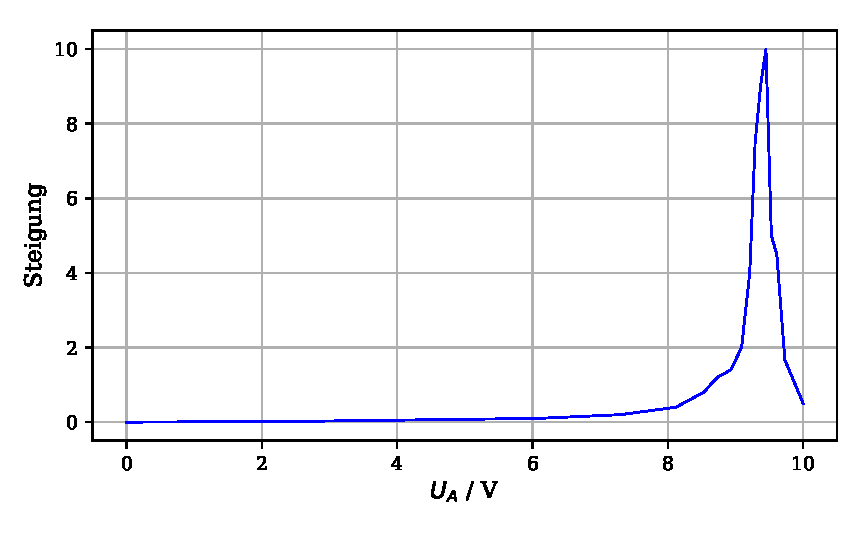
\includegraphics{plota1.pdf}
  \caption{Die Energieverteilung der Elektronen bei einer Temperatur von $T=299,25$K.}
  \label{fig:plot}
\end{figure}

\begin{table}[H]
  \centering
  \caption{Werte für den Graphen für die Bestimmung der Energieverteilung bei einer Temperatur $T=418,15$K.}
  \label{tab:Parameter}
  \begin{tabular}{c c}
    \toprule
    Steigung $m$ &  Genortme Spannungen \\
    \bottomrule
    0 & 0\\
    0 & 2,57\\
    2,82 & 3,94\\
    1,8 &4,35\\
    1,4 &4,55\\
    0,4 &4,75\\
    0,2 &5,16\\
    0,1 &5,57\\
    0,2&6,39\\
    0,27 &9,25\\
    0 &10\\
  
    \bottomrule
  \end{tabular}
\end{table}

Der Graph zu dieser Messreihe ist in Abbildung () zu finden.

\begin{figure}[H]
  \centering
  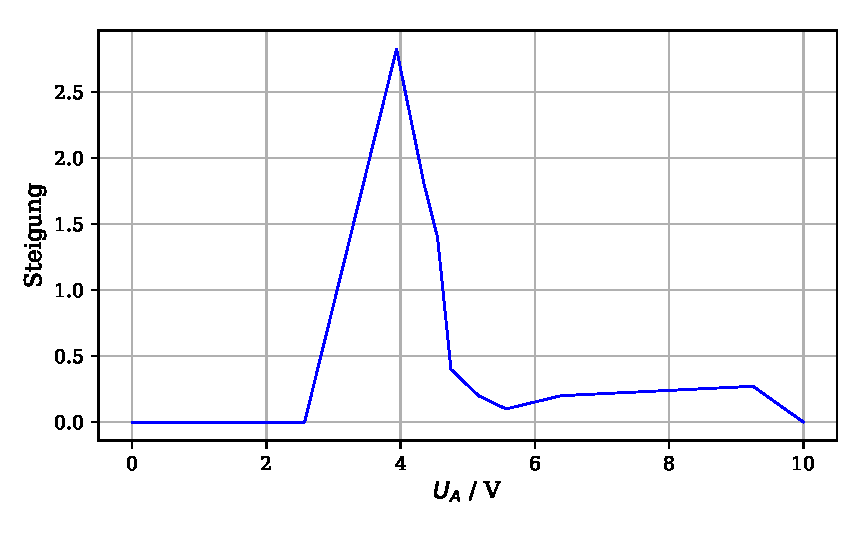
\includegraphics{plota2.pdf}
  \caption{Die Energieverteilung der Elektronen bei einer Temperatur von $T=418,15$K.}
  \label{fig:plot}
\end{figure}

\noindent Aus Abbildung () kann man das Kontaktpotential ablesen. 
An dem Maximum des Graphen ist die Energie der Elekronen $9,45\si{\eV}$.
Energie der elektronen 9,45.Da die Beschleunigungsspannung von $11\si{\V}$ hinzugerechnet werden muss, ergibt sich
ein Kontaktpotential von $K_1 = 1,55 \si{\V}$.
Damit viele Zusammenstöße der Elektronen mit den Quecksilber-Atomen stattfinden können, muss die mittlere freie Weglänge klein gegen den Abstand $a$ sein.
Somit treten mehr Stöße bei der ersten Messreihe auf.
Im nächsten Abschnitt wird klar, dass die Anregungsspannung bei ca. $ (4,89 \pm 0,206) \si{\V}$ liegt. Dies lässt das Gefälle in Abbildung () erklären.

\begin{figure}[H]
  \centering
  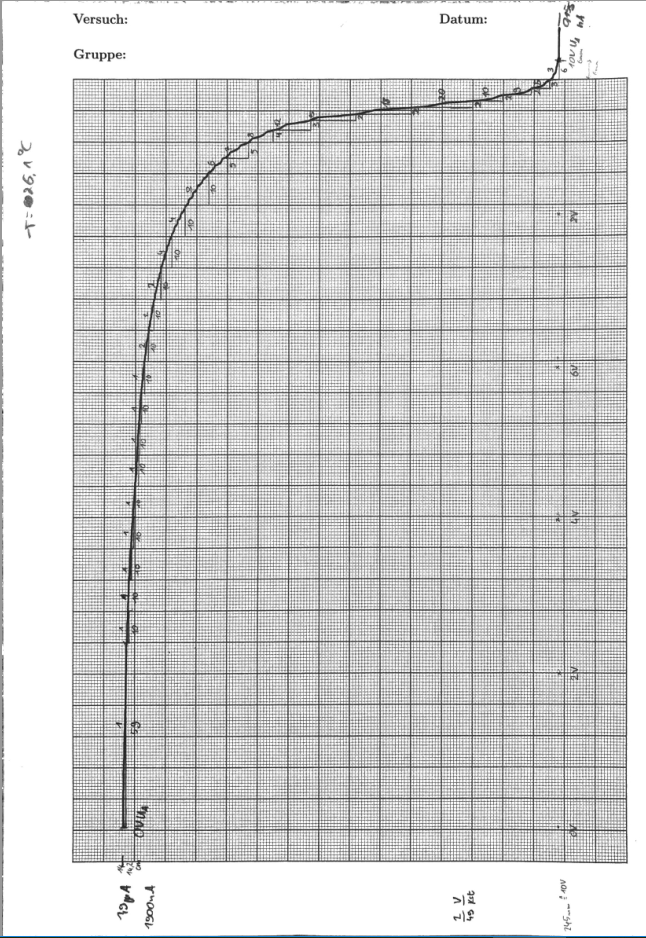
\includegraphics{a.PNG}
  \caption{Erstellte Kurve bei einer Temperatur von $T=299,25$K. }
  \label{fig:plot}
\end{figure}
\begin{figure}[H]
  \centering
  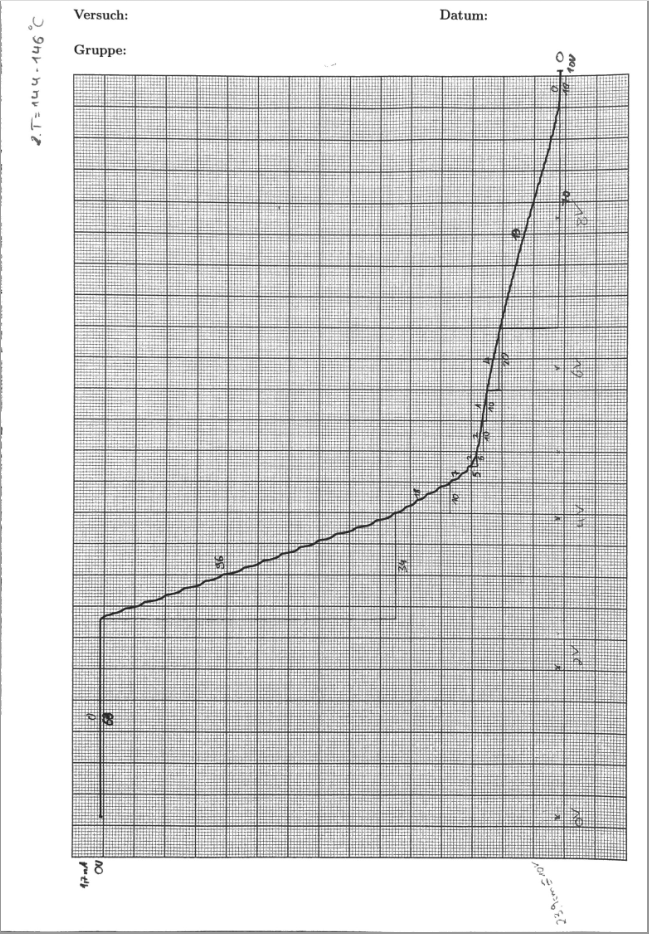
\includegraphics{b.PNG}
  \caption{Erstellte Kurve bei einer Temperatur von $T=418,15$K.}
  \label{fig:plot}
\end{figure}

\subsection{Analyse der Franck-Hertz-Kurve}
Die Franck-Hertz-Kurve für eine Temperatur von ca. $T=472,15 \si{\K}$ ist in Abbildung () zu sehen.
Aus dieser werden die Abstände der Maxima gemessen, zu sehen in Tabelle (4).

\begin{table}[H]
  \centering
  \caption{Abstände der Maxima der Franck-Hertz-Kurve.}
  \label{tab:Parameter}
  \begin{tabular}{c }
    \toprule
     Abstand der Maxima in V \\
    \bottomrule
     4,945\\
     4,670\\
     4,670\\
     4,670\\
     4,945\\
    4,670\\
    4,945\\
    5,220\\
     4,945\\
    5,220\\
   \bottomrule
  \end{tabular}
\end{table}

Der gemittelte Abstand beträgt
\begin{align*}
U_1 = (4,89 \pm 0,206) \si{\V}.
\end{align*}
Nach Gleichung () ist die 1. Anregungsenergie
\begin{align*}
E_1 = U_1 \cdot e_0 = (7,83 \pm 0,33)\cdot 10^{-19} \si{\J} \\
E_1 = (4,89 \pm 0,206) \si{\eV}.
\end{align*}
Alle Mittelwerte und Fehler werden mit Python berechnet.
Aus dem Abstand wird nun die Wellenlänge der emittierten Strahlung mit Hilfe von Formel () und der Relation $\lambda = \frac{c}{\nu} $ berechnet.
\begin{align*}
\nu = \frac{E_1}{h} = (1,18 \pm 0,05)\cdot 10^{-15} \si{\Hz}\\
\lambda = (2,54 \pm 0,11)\cdot 10^{23} \si{\m}.
\end{align*}
Inelastische Stöße treten nur auf, wenn die Energie hoch genug ist.
Der Energieverlust beim elastischen Stoß ist also zu vernachlässigen.

\begin{figure}[H]
  \centering
  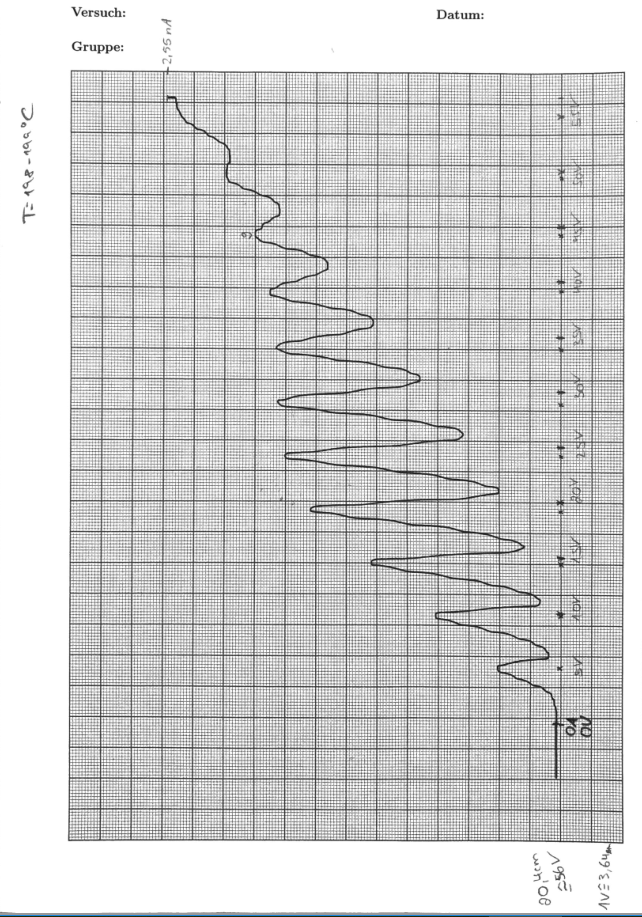
\includegraphics{FranckHertz.PNG}
  \caption{Franck-Hertz Kurve bei einer Temperatur von $T=472,15 \si{\K}$.}
  \label{fig:plot}
\end{figure}


\subsection{Bestimmung der Ionisierungsspannung von Quecksilber}
Bei diesem Versuchsteil betrug die Temperatur $T= 377,15\si{\K}$.
Aus der angefügten Abbildung () lässt sich der Wert $U_{ion}+K$ ablesen.
Dazu wird eine Asymptote eingezeichnet und der Schnittpunkt mit der x-Achse abgelesen.
Er beträgt $X = 2,5 \si{\V}$. Mit Hilfe des vorher bestimmten Kontaktpotentials, wird die Spannung bestimmt.
\begin{align*}
U_{ion} = X-K_1 = 0,95\si{\V}.
\end{align*}

\begin{figure}[H]
  \centering
  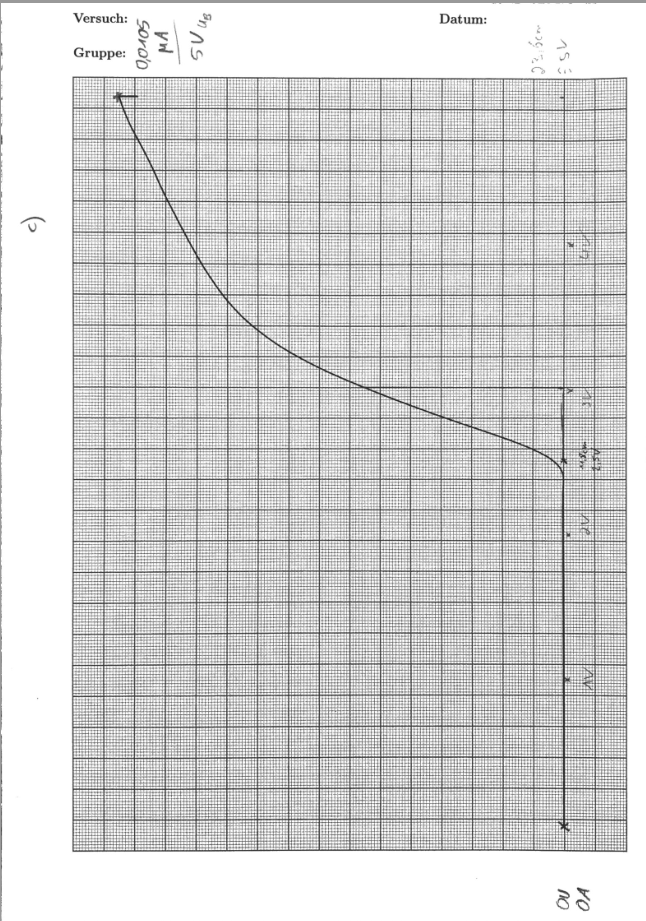
\includegraphics{c.PNG}
  \caption{Beschleunigungsspannung und Strom bei Ionisierung bei einer Temperatur von $T= 377,15\si{\K}$.}
  \label{fig:plot}
\end{figure}
